\section{Multilayer Perceptron}

Eines der bekanntesten Architekturen der neuronalen Netze ist das sogenannte \emph{Multilayer Perceptron}. Diese sehr vielfältig eingesetzte Struktur verwendet den erläuterten Backpropagation-Lernalgorithmus und erzielt damit in der Regel sehr gute Ergebnisse. Beim MLP spielt die Aktivierungsfunktion durchaus auch eine tragende Rolle und ist nicht fest definiert (häufig wird jedoch die Sigmoid-Funktion verwendet). Wenn das Netzwerk sehr viele verborgene Zwischenschichten besitzt wird es allgemein als \emph{tief} bezeichnet und es kann zu Problemen beim Training kommen. Hierbei gibt es spezielle Techniken die diese Probleme lösen können und generell unter dem Namen \emph{depplearning} zusammengefasst werden. Da diese Architektur als so vielfältig gilt kann sie in vielen verschiedenen Anwendungsbereichen eingesetzt werden, hier ein paar Beispiele: 

\begin{multicols}{2}
\begin{itemize}
\item Mustererkennung 
\item Funktionenapproximation
\item Klassifizierung
\item Prognose
\item Diagnose
\item Steuerung 
\item Optimierung
\end{itemize}
\end{multicols}

\paragraph{Zusammenfassung - Aufbau}

Da diese Architektur als Grundlage für die Erklärung des Backpropagation-Algorithmus gewählt wurde folgt nur eine kurze Zusammenfassung des Aufbaus. Für eine ausführliche Erklärung sämtlicher Notations-Regeln etc. siehe Abschnitt \ref{ss:notationBP}. 

Diese Struktur gilt als mehrschichtige vorwärtsgekoppeltes Netzwerk. Teilweise wird sie auch als Mehrschichten-Perzeptron bezeichnet weil sie einem Perzeptron-Netzwerk mit mehreren Schichten sehr ähnelt. Dieses Netzwerk besteht aus einer Eingabeschicht, einer oder mehrerer innerer Schichten\footnote{in englisch auch häufig \emph{hiden Layers} genannt}, und einer Ausgabeschicht. 

\begin{figure}[!htb]
	\centering
	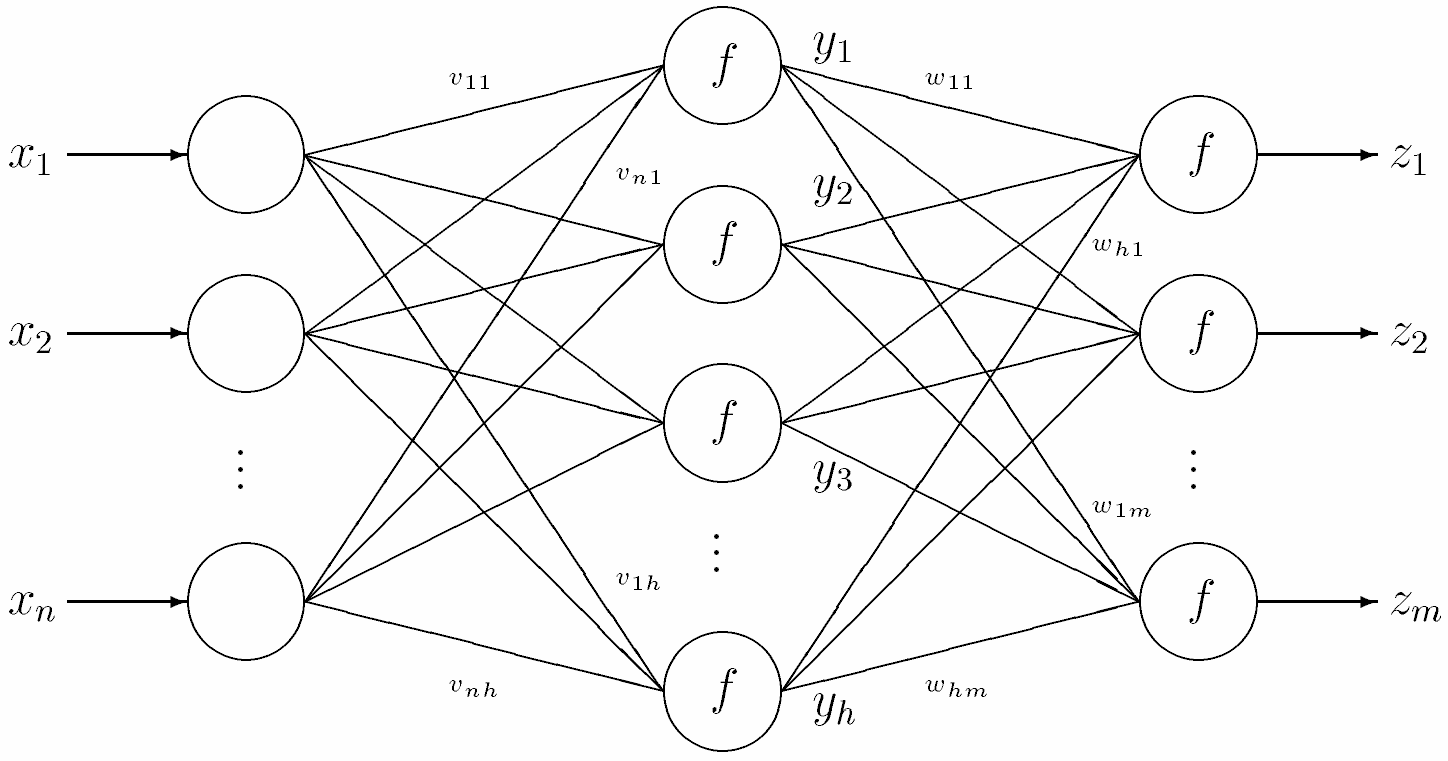
\includegraphics[width=.8\linewidth]{./img/mlp1}
	\mycaption{MLP - Aufbau}{ss}
	\label{fig:mlpAufbau}
\end{figure}

Das Netz kann \emph{n} Eingabewerte annehmen, welche jeweils mit den Neuronen $x_1$ bis $x_n$ entgegengenommen werden. Die einzelnen Neuronen werden mit einer Aktivierungsfunktion belegt und verwenden intern einen eigenen Schwellwert. Das durch-iterieren diverser Eingabewerte wird auch als \emph{Feedforward} bezeichnet, wobei am Ende \emph{m} Ausgabewerte entstehen die über die Ausgabeneutronen der letzten Schicht weitergeleitet werden (siehe $z_1$ bis $z_n$). 

\FloatBarrier

\paragraph{Aktivierungsfunktionen}

\subparagraph{Sigmoid}
Um beim Backpropagation-Algorithmus die ersten Ableitungen der Aktivierungsfunktion berechnen zu können müssen diese stetig differenzierbar sein. Eine häufig verwendete Funktion ist die \emph{Sigmoid}-Funktion. Diese logistische Funktion zeichnet sich durch aus, dass alle möglichen Eingabewerte einen Ausgabewert zwischen 0 und 1 generieren. Sehr kleine Werte streben dabei gegen 0 während sehr große Werte gegen 1 streben. Die Formel sieht folgendermaßen aus: 

\begin{equation}
f(x) = \frac{1}{1 + exp(-b * x)}
\end{equation}
 
Die Konstante \emph{b} beschreibt dabei die Steilheit der Kurve. Die Ableitung der Funktion besitzt die Form $f'(x) = b * f(x)(1-f(x))$.

\begin{figure}[!htb]
	\centering
	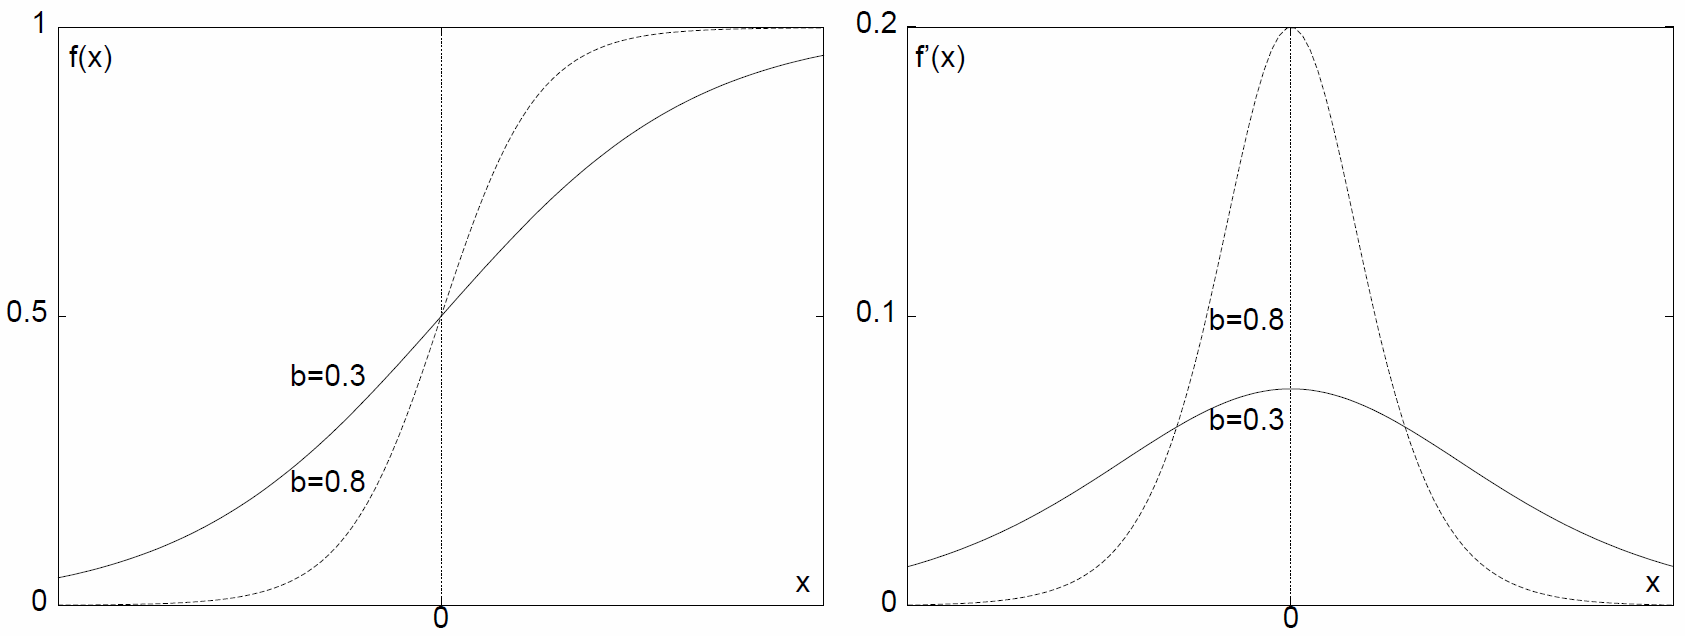
\includegraphics[width=.8\linewidth]{./img/plotSigmoid}
	\mycaption{Sigmoid - Plot}{ss}
	\label{fig:mlpSigmoid}
\end{figure}



% \subparagraph{Tangens Hyperbolicus}

% Die Funktion wird auch häufig als Aktivierungsfunktion verwendet und besitzt die Gleichung sowie die Ableitungen: 

% \begin{equation}
% f(x) = tanh(x) = \frac{2}{1+exp(-2x}-1
% \end{equation}

% \begin{equation}
% f'(x) = 1 - tanh^2(x)
% \end{equation}

